\documentclass[11pt, oneside]{article}  
\usepackage[margin=0.5in]{geometry} % Margins
\usepackage[ampersand]{easylist} % Bullets for lists
\usepackage[bottom]{footmisc}  % Glue footnotes to bottom
\usepackage{graphicx}
\graphicspath{ {imgs/} }

\title{Operating Systems Principles\\UCLA-CS111-W18}
\author{Quentin Truong\\Taught by Professor Reiher}
\date{Winter 2018}


\begin{document}
\maketitle
\tableofcontents
\pagenumbering{arabic}
\clearpage


%========================================================
\section{L3: Arpaci-Dusseau Chapter 5: Interlude: Process API}
\subsection{The fork() System Call}
	\begin{easylist}  
	\ListProperties(Hide=100, Hang=true, Progressive=4ex, Style*=--\ , Style2*=$\bullet\ $)
        & Crux: How to create and control processes
		& fork()
        && Creates new process; returns child's PID to parent; returns 0 to child;
        && Each has own PC, registers, address space
        & Nondeterministic Behavior
        && Scheduler will decide which process to run
        && May lead to problems in multi-threaded programs
	\end{easylist}

\subsection{The wait() System Call}
    \begin{easylist}  
    \ListProperties(Hide=100, Hang=true, Progressive=4ex, Style*=--\ , Style2*=$\bullet\ $)
        & wait()
        && Parent calls wait() to wait for child to finish execution
    \end{easylist}

\subsection{The exec() System Call}
    \begin{easylist}  
    \ListProperties(Hide=100, Hang=true, Progressive=4ex, Style*=--\ , Style2*=$\bullet\ $)
        & exec()
        && Loads code, overwrites code segment, and reinitializes memory space
        && Takes exceutable name and arguments
        && Does not create a new process; transform current process
    \end{easylist}

\subsection{Why? Motivating The API}
    \begin{easylist}  
    \ListProperties(Hide=100, Hang=true, Progressive=4ex, Style*=--\ , Style2*=$\bullet\ $)
        & Separation
        && Separating fork() and exec() allows code to alter the environment of the about-to-run program
        & Example
        && Shell forks a process, execs the program, and waits until finished
        && The separation allows for things such as output to be redirected (closes stdout and opens file)
    \end{easylist}

\subsection{Other Parts Of The API}
    \begin{easylist}  
    \ListProperties(Hide=100, Hang=true, Progressive=4ex, Style*=--\ , Style2*=$\bullet\ $)
        & kill()
        && System call sends signal to process to sleep, die, etc
    \end{easylist}
%========================================================

%========================================================
\section{L3: Arpaci-Dusseau Chapter 6: Mechanism: Limited Direct Execution}
\subsection{Basic Technique: Limited Direct Execution}
    \begin{easylist}  
    \ListProperties(Hide=100, Hang=true, Progressive=4ex, Style*=--\ , Style2*=$\bullet\ $)
        & Crux: How to efficiently virtualize CPU with control
        & Limited Direct Execution
        && OS will create entry for process list, allocate memory for program, load program into memory, setup stack with argc/v, clear registers, execute call to main()
        && Program will run main(), execute return
        && OS will free memory, remove from process list
        & LDE good bc fast, but
        && Problem of keeping control
        && Problem of time sharing still
    \end{easylist}

\subsection{Problem 1: Restricted Operations}
    \begin{easylist}  
    \ListProperties(Hide=100, Hang=true, Progressive=4ex, Style*=--\ , Style2*=$\bullet\ $)
        & User mode vs. Kernel mode
        && Restricted mode which needs to ask kernel to perform system calls
        && Calls like open() are actually procedure calls with trap to enter kernel and raise privilege
        && Return-from-trap is used to enter user mode from kernel and drop privilege
        && Push counters, flags, registers onto per-process kernel stack when trapping
        & Trap table is used to control what code is executed when trapping
        && Trap handler used by hardware to cause interrupts 
        && Telling hardware where trap table is is privileged
        && Trap handler actually uses system-call number, rather than specifying an address (another layer of protection)
        & Two phases of LDE
        && At boot, kernel initializes trap table and remembers where it is
        \begin{figure}[h]
            \centering
            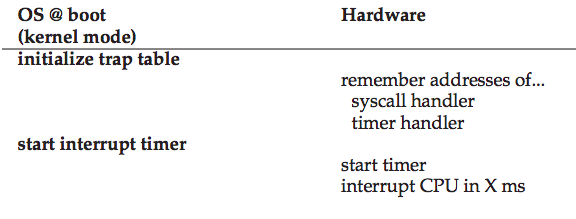
\includegraphics[scale=0.6]{boot}
        \end{figure}
    \end{easylist}

\subsection{Problem 2: Switching Between Processes}
    \begin{easylist}  
    \ListProperties(Hide=100, Hang=true, Progressive=4ex, Style*=--\ , Style2*=$\bullet\ $)
        & How can OS regain control?
        && Because process is running, so OS is not running
        & Cooperative Approach
        && System calls include explicit yield system call, transfering control back to OS
        & Noncooperative Approach
        && Reboot, Timer Interrupt
        & Saving and Restoring Context
        && Scheduler will choose when to switch processes
    \end{easylist}
    \begin{figure}[h]
        \centering
        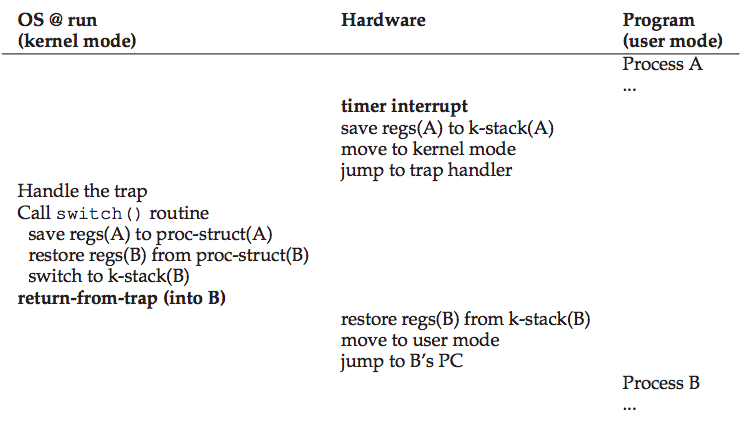
\includegraphics[scale=0.5]{context_switch}
    \end{figure}

\subsection{Worried About Concurrency?}
    \begin{easylist}  
    \ListProperties(Hide=100, Hang=true, Progressive=4ex, Style*=--\ , Style2*=$\bullet\ $)
        & Interrupt during interrupt?
        && Many complex things to do
        && Could disable interrupts (but this might lose interrupts), or locking schemes, etc
    \end{easylist}

\subsection{Summary}
    \begin{easylist}  
    \ListProperties(Hide=100, Hang=true, Progressive=4ex, Style*=--\ , Style2*=$\bullet\ $)
        & Reboot
        && Good technique because restores system to well-tested state
        && OS will 'baby-proof' by only allowing processes to run in restricted mode and with interrupt handlers
    \end{easylist}
%========================================================

%========================================================
\section{L3: Linking and Libraries: Object Modules, Linkage Editing, Libraries}
\subsection{Overview}
    \begin{easylist}  
    \ListProperties(Hide=100, Hang=true, Progressive=4ex, Style*=--\ , Style2*=$\bullet\ $)
        
    \end{easylist}
%========================================================

%========================================================
\section{L3:}
\subsection{Overview}
    \begin{easylist}  
    \ListProperties(Hide=100, Hang=true, Progressive=4ex, Style*=--\ , Style2*=$\bullet\ $)
        
    \end{easylist}
\clearpage

\end{document}  